\section{Projection of the Measurement}
\subsection{Kinematic Coverage}
\begin{figure}[!ht]
 \begin{center}
      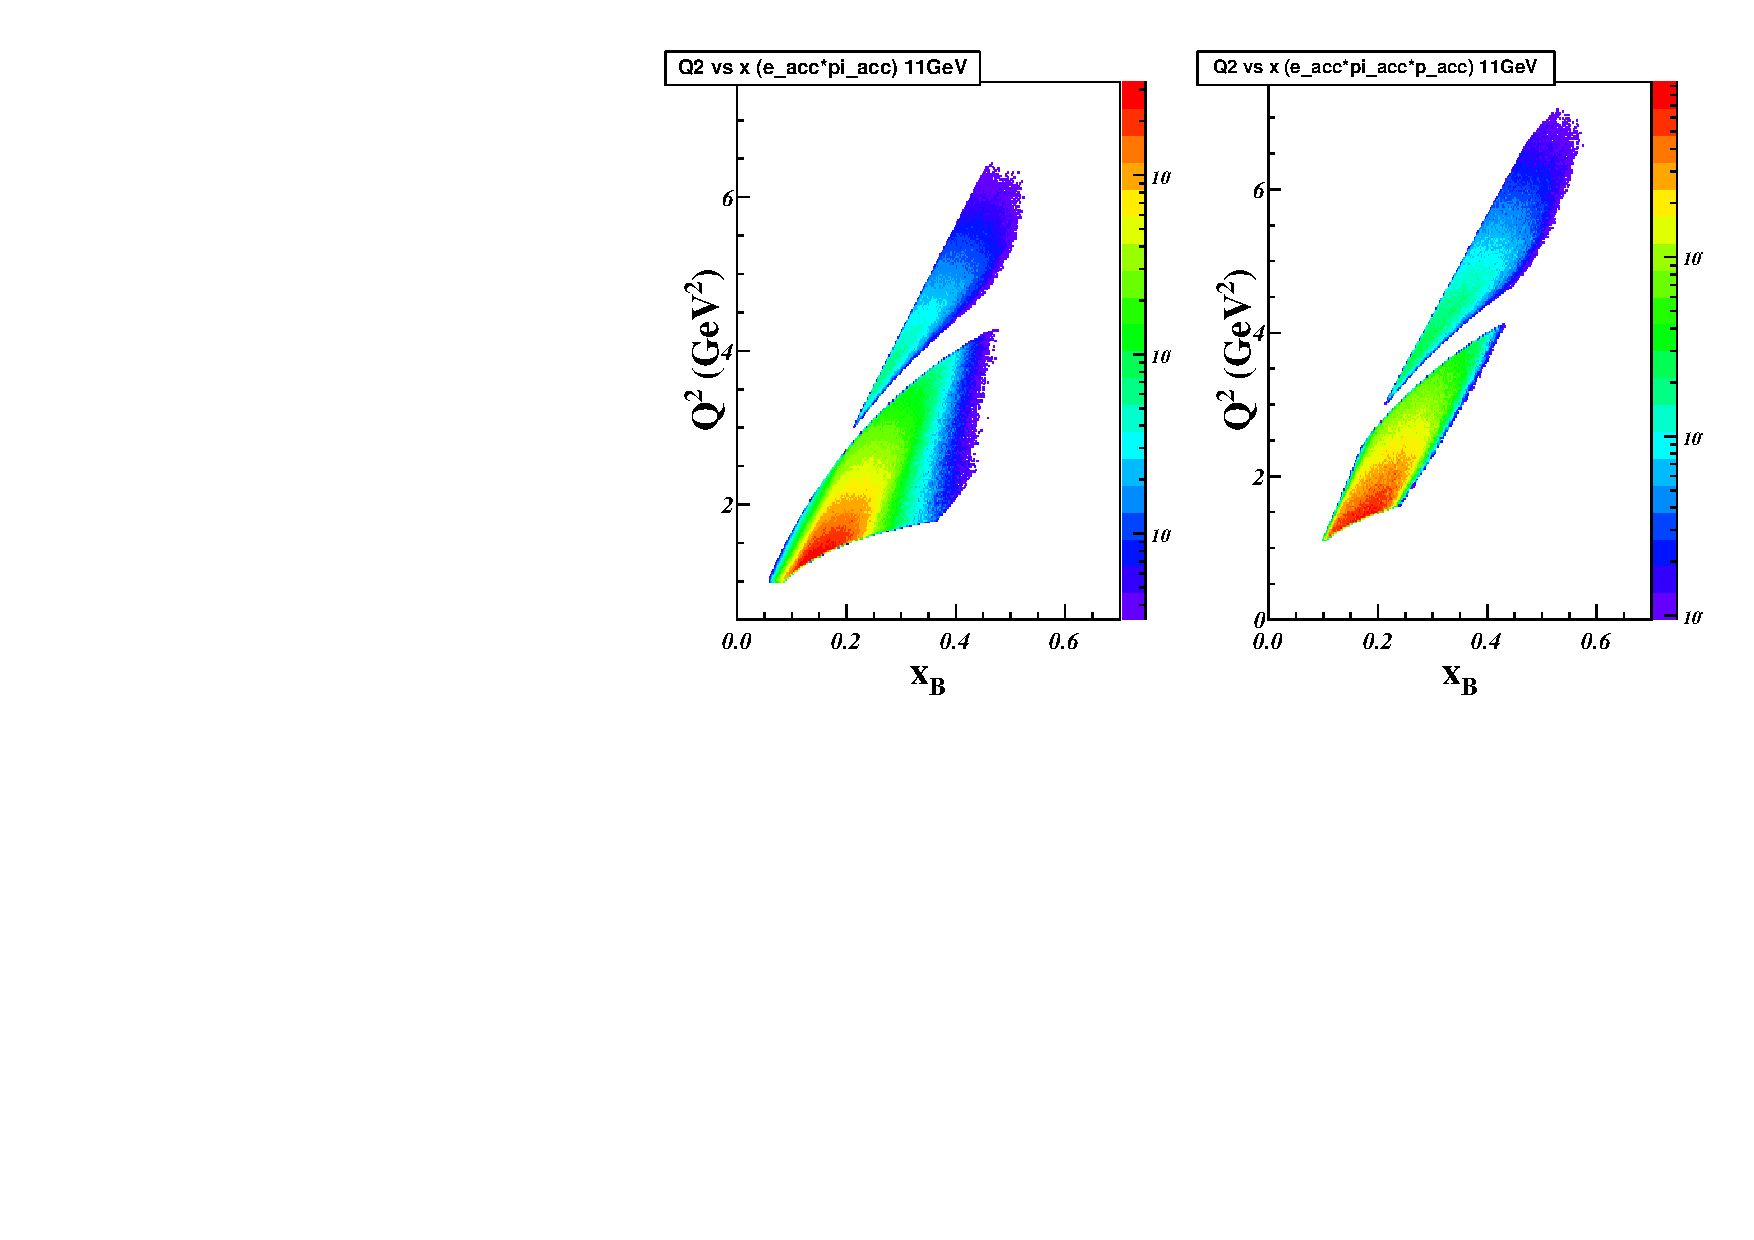
\includegraphics[type=pdf, ext=.pdf,read=.pdf,width=0.6\textwidth]{./figures/E11_Q2_x_epip_Q2gt1}
 \caption[The kinematic coverage at different acceptances]{\footnotesize{The kinematic coverage at different acceptances at $11~GeV$. The left plot shows the coverage when detecting all recoil protons, while the right plot shows the coverage with proton detection by existing SoLID detectors. Colors correspond to rates (Hz) in log scale.}}
  \label{kin_cor}
  \end{center}
\end{figure}
\begin{figure}[!ht]
 \begin{center}
    \subfloat[w/ $\mathrm{Q^{2}>1~GeV^{2}}$ cut]{
      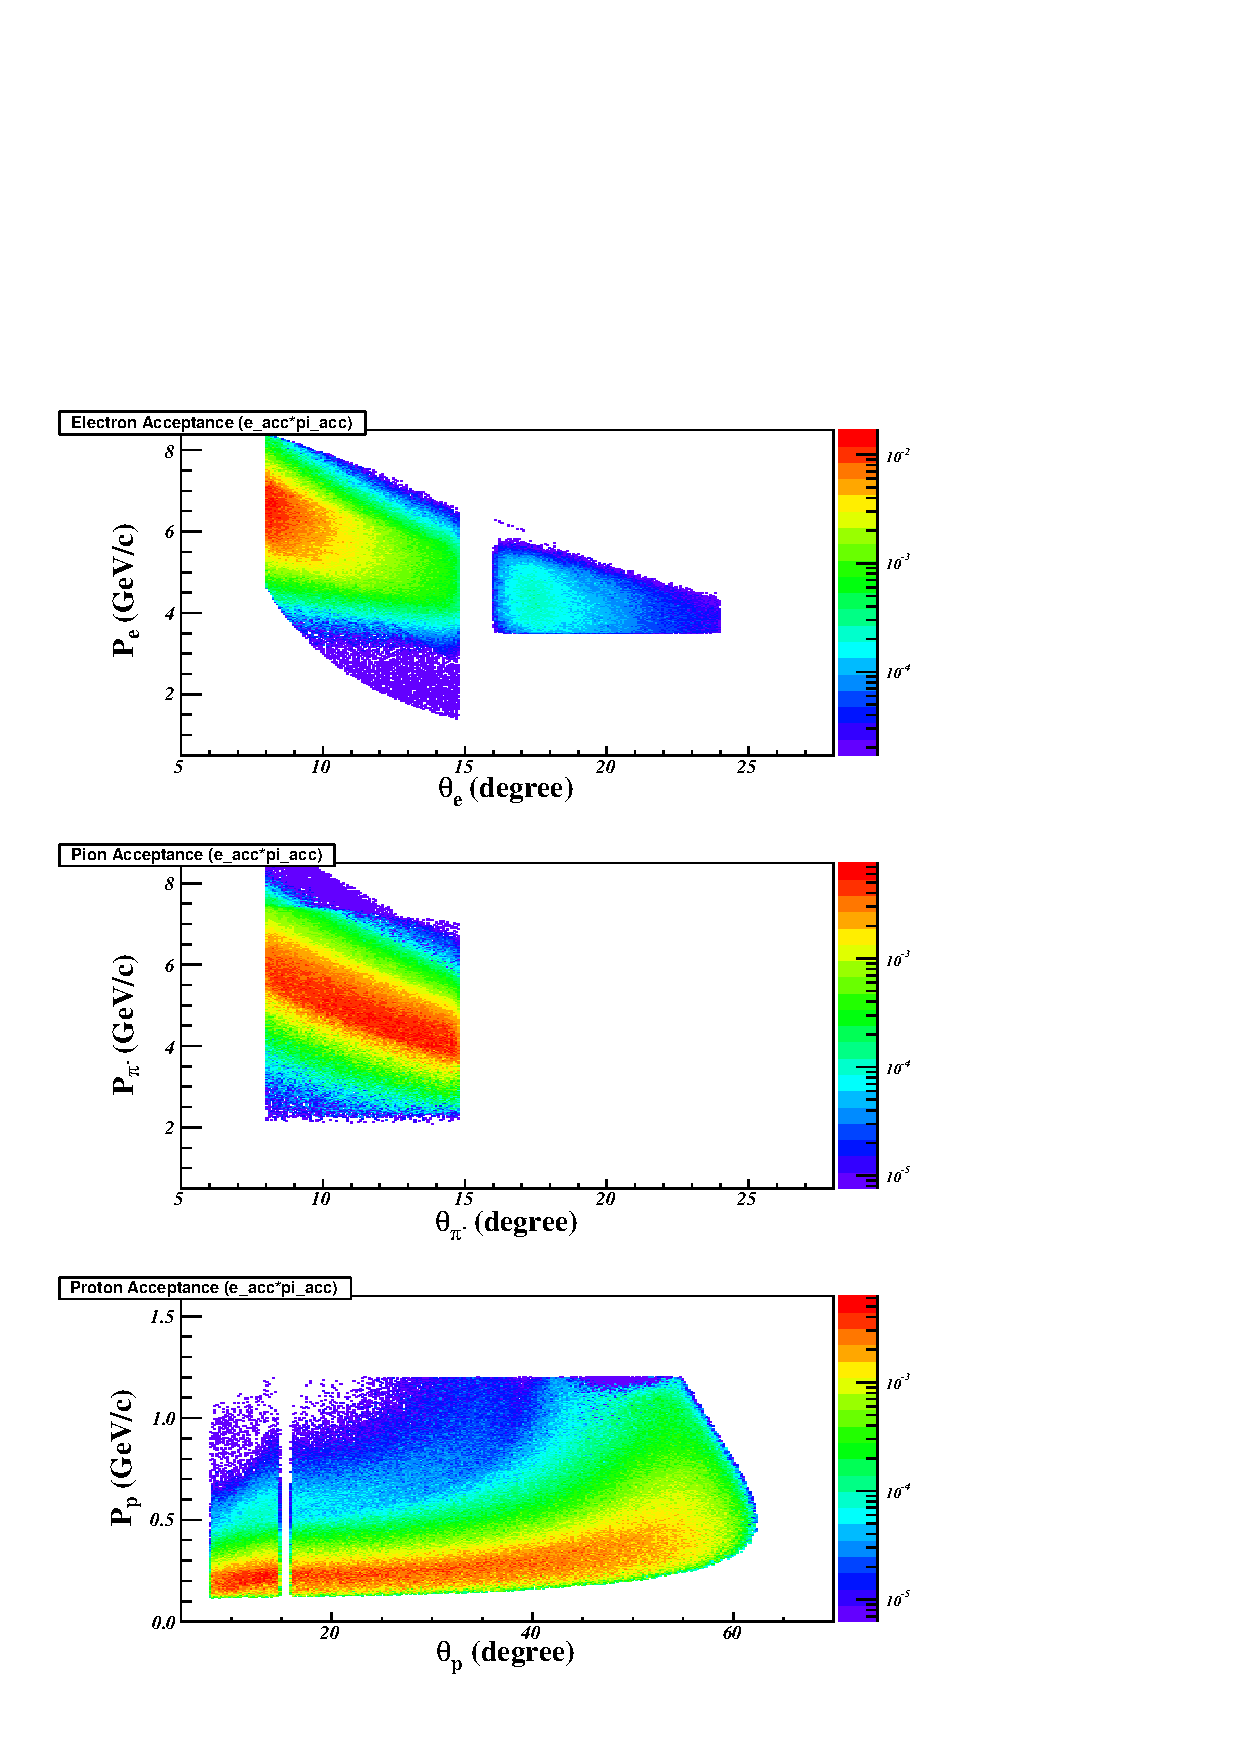
\includegraphics[type=pdf, ext=.pdf,read=.pdf,width=0.35\textwidth]{./figures/E11_acc_epi}
    }
     \subfloat[w/ $\mathrm{Q^{2}>4~GeV^{2}}$ cut]{
      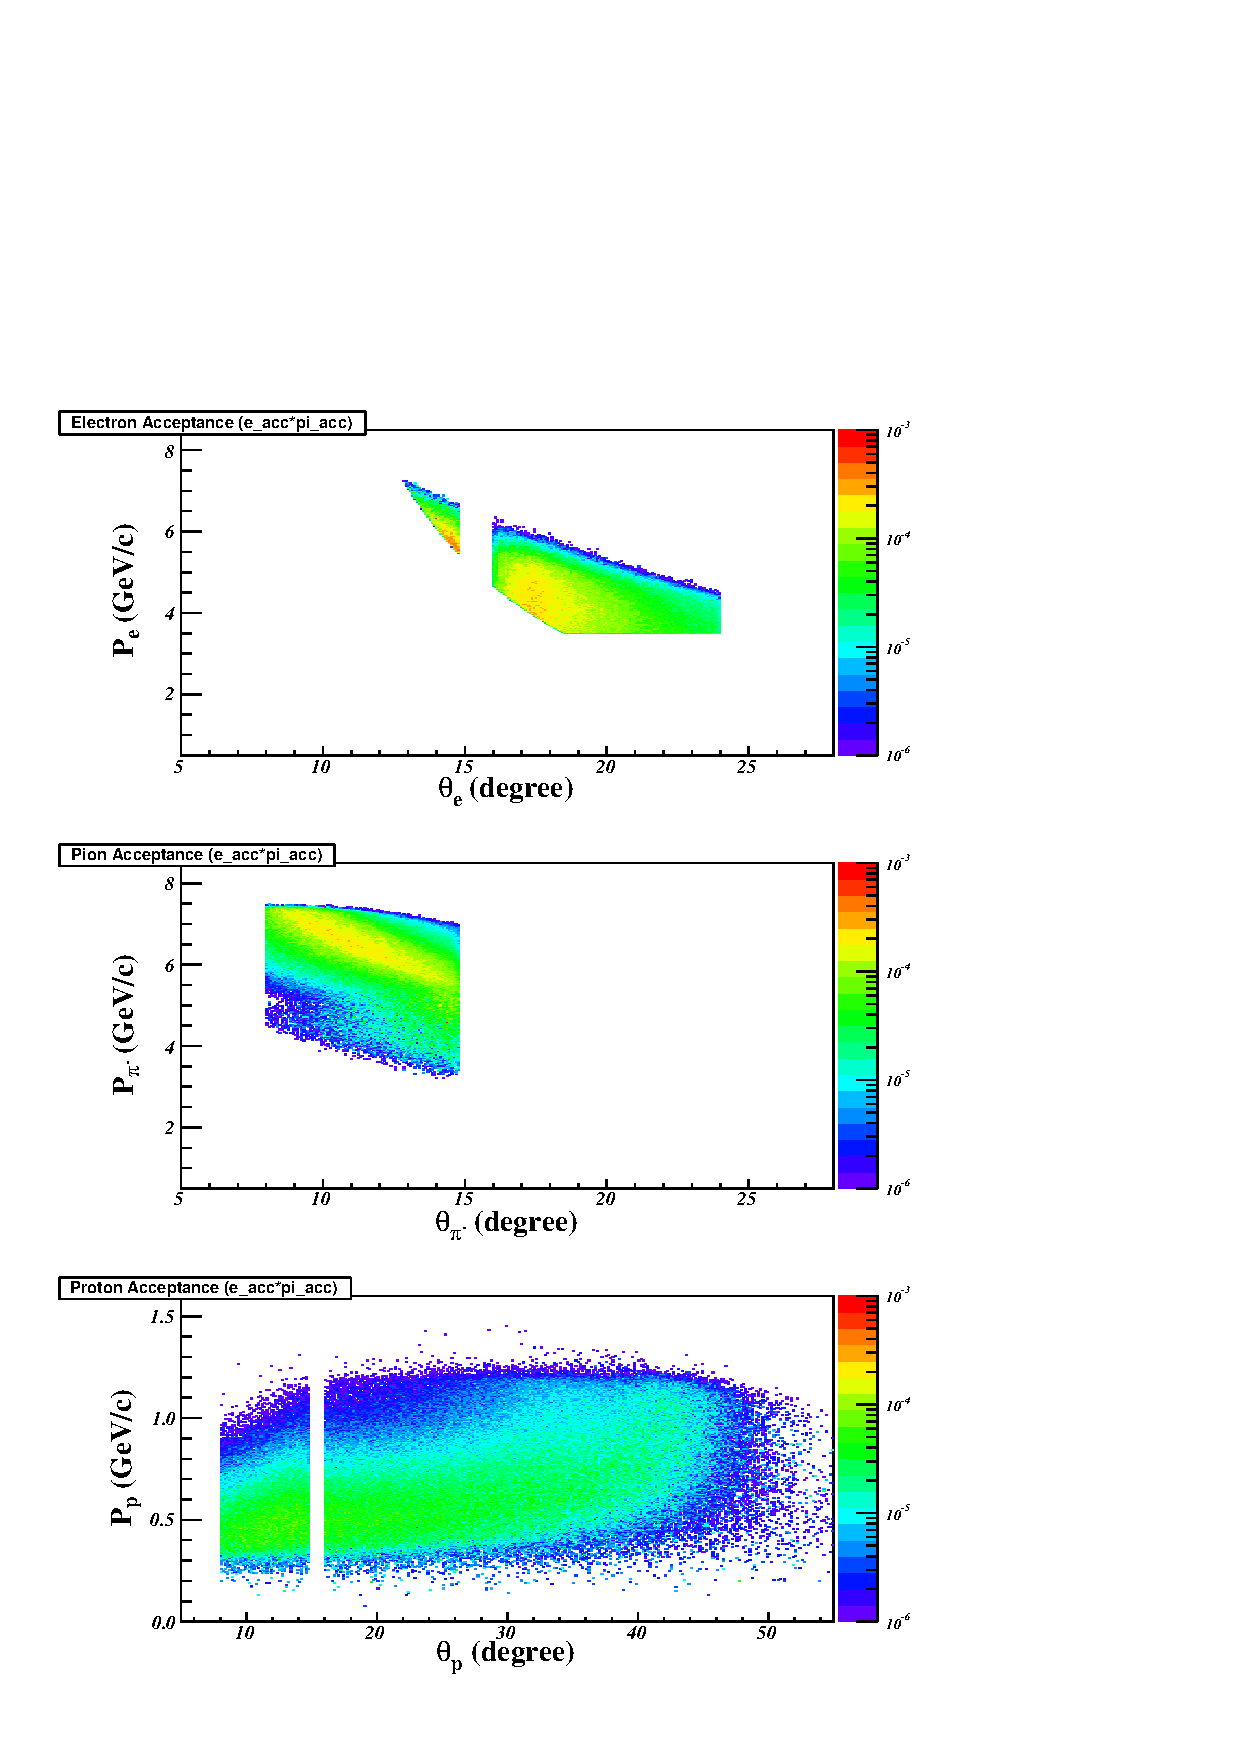
\includegraphics[type=pdf, ext=.pdf,read=.pdf,width=0.35\textwidth]{./figures/E11_acc_epi_Q2gt4}
    }
   \caption[The acceptance of the momenta and scattering angles for electrons, $\pi^{-}$ and protons]{\footnotesize{The acceptance of the momenta and polar angles at two different $\mathrm{Q^{2}}$ cuts. In each panel, the top, middle and bottom plots are for electrons, $\pi^{-}$ and protons, respectively. The distribution of protons is given by assuming we detect all recoil protons. Colors correspond to rates (Hz) in log scale.}}
  \label{p_theta}
  \end{center}
\end{figure}
\begin{figure}[!ht]
 \begin{center}
    \subfloat[w/ $\mathrm{Q^{2}>1~GeV^{2}}$ cut]{
      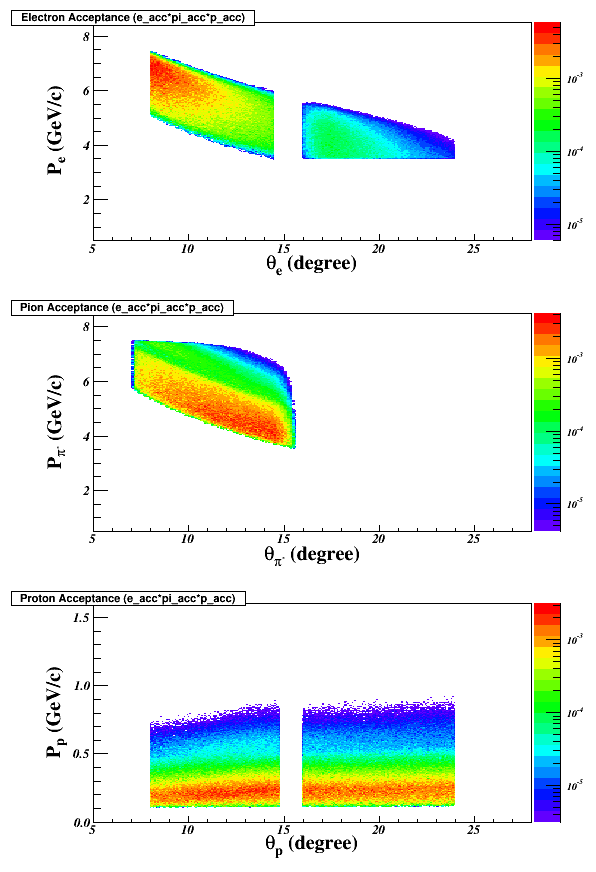
\includegraphics[type=pdf, ext=.pdf,read=.pdf,width=0.35\textwidth]{./figures/E11_acc_epip}
    }
     \subfloat[w/ $\mathrm{Q^{2}>4~GeV^{2}}$ cut]{
      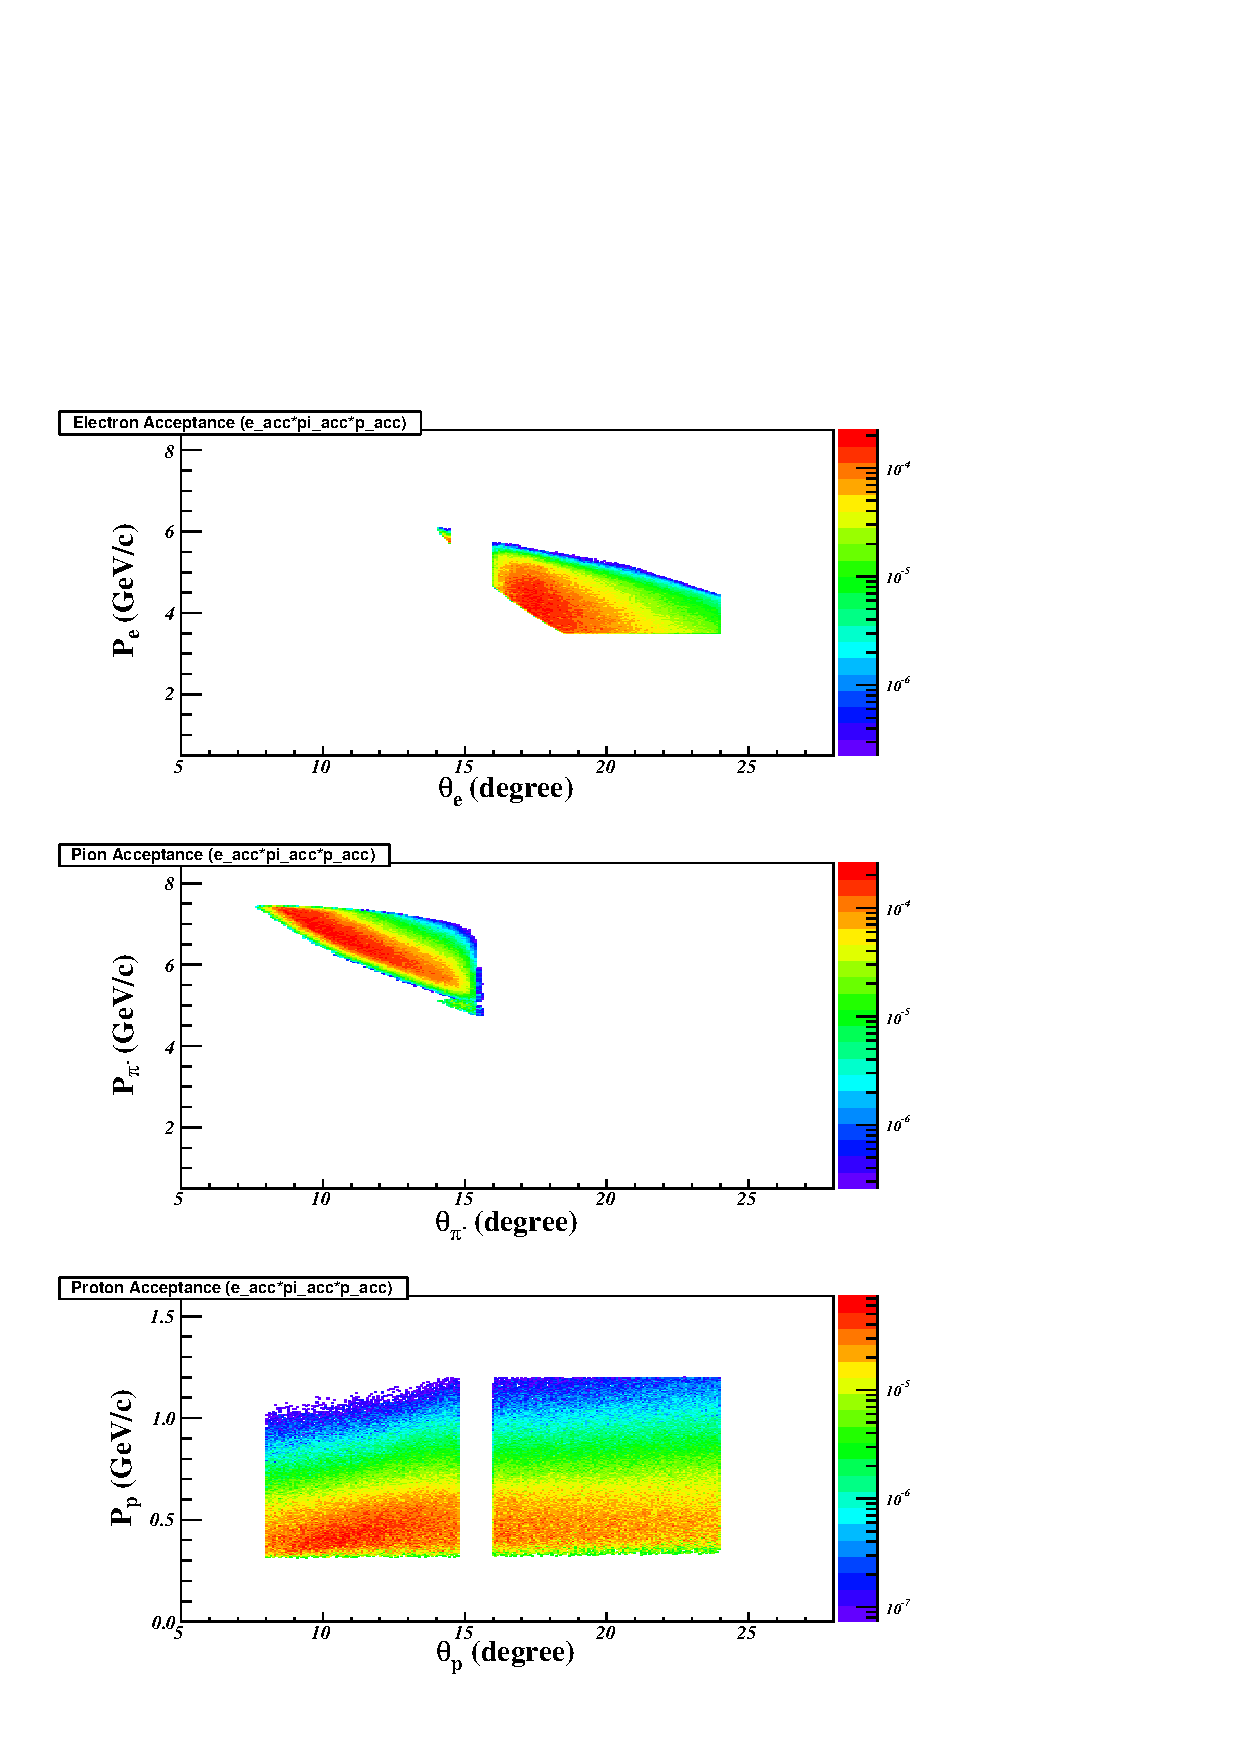
\includegraphics[type=pdf, ext=.pdf,read=.pdf,width=0.35\textwidth]{./figures/E11_acc_epip_Q2gt4}
    }
   \caption[The acceptance of the momenta and scattering angles for electrons, $\pi^{-}$ and protons when only detecting small angle protons]{\footnotesize{The acceptance of the momenta and polar angles  at two different $\mathrm{Q^{2}}$ cuts  when only detecting small angle protons with the existing SoLID detectors. In each panel, the top, middle and bottom plots are for electrons, $\pi^{-}$ and protons, respectively. The distribution of protons is given by assuming we detect all recoil protons. Colors correspond to rates (Hz) in log scale.}}
  \label{p_theta1}
  \end{center}
\end{figure}
The kinematic coverage in $Q^{2} vs. x_{B}$ is shown in Fig.~\ref{kin_cor} where two proton detection cases were given: (a) by using  existing SoLID detectors to detect protons at small angles ($8^{\circ}\sim24^{\circ}$) and adding a new proton recoil detector to detect rest of recoil protons at large angle ($24^{\circ}\sim65^{\circ}$), or (b) by only using the existing SoLID detectors. These distributions were weighted by the DVMP cross sections and the spectrometer acceptance obtained from the GEANT4 simulation with the SIDIS configuration. As shown in these plots, the range of $Q^{2}$ is from 1.0~$GeV^{2}$ to 8.0~$GeV^{2}$, $x_{B}$ goes from 0.1 up to 0.75.   

Fig.~\ref{p_theta} shows the momentum and angular acceptance of electrons, $\pi^{-}$ and protons which form the DVMP events and can be detected in SoLID. Since most of valid DVMP events are at high $Q^{2}$, a cut of $\mathrm{Q^{2}>4~GeV^{2}}$ is applied to see how it changes the acceptance. The recoil protons shown in Fig.~\ref{p_theta}  have low momenta ranged from 0.3~GeV/c up to 1.2~GeV/c and their rates distribute near uniformly along the scattering angle. Fig.~\ref{p_theta1} shows the change of acceptance for all particles when only using the existing SoLID detectors to detect small angle protons.

\subsection{Estimated Rates}
\begin{table}[!ht]
\centering
\begin{tabular}{|c|c|c|}
 \hline
  $\mathrm{1<Q^{2}<4~GeV^{2}}$             &    $\mathrm{Q^{2}>4~GeV^{2}}$  & Total\\
 \hline
                  \multicolumn{3}{|c|}{DVMP: $\vec{n}(e,e'\pi^{-})p$ Triple-Coincidence (Hz)}     \\
 \hline
 17.79 (0.22)   &  0.53 (0.31) & 26.45 (7.66)   \\
 \hline
                  \multicolumn{3}{|c|}{SIDIS: $\vec{n}(e,e'\pi^{-})X$ Double-Coincidence (Hz)}                                     \\
 \hline
1388.85 & 35.77 & 1424.62   \\
 \hline
\end{tabular}
\caption[Triple-Coincidence rates for neutron-DVMP]{\footnotesize{Triple-Coincidence  rates for DVMP events compared with the SIDIS rates. Numbers in brackets are the DVMP rates with only detecting protons using existing SoLID detectors. The online production trigger will be the SIDIS double-coincidence trigger of which rates are also given.}}
\label{rate_table}
\end{table} 
Table~\ref{rate_table} lists the triple-coincidence rate of the DVMP events. The rates were calculated with the simulated events weighted by the target luminosity, the SoLID acceptances and cross sections. The rates are the unpolarized event rates and are not corrected by the beam and target polarization, target dilution and so on. The total integrated physics rate is estimated to be around 26~Hz  at 11~GeV, or  0.53 Hz at $\mathrm{Q^{2}>4~GeV^{2}}$. If only using the existing SoLID detectors to detect protons, the rate drops to 0.31 Hz at $\mathrm{Q^{2}>4~GeV^{2}}$.  For comparing,  the table also gives the SIDIS rate  which will be the online production trigger rates and is the main background of the DVMP events. 

\subsection{Asymmetry Projections}
The proposed new experiment will run in parallel with E12-10-006 of which total beam time of 48 days at $E_{0}=11~GeV$ has been approved.  

The number of events ($N$) in each bin is calculated with the total simulated events after applying cuts on the corresponding ranges of these 4 variables. As shown in Eq.~\ref{ncount}, each event in one bin is then corrected by the weight of the cross section and the acceptance value of the electron and the photon. $N$ is further normalized by the phase-space ($PSF$), total generated events ($N_{gen}$), beam-time ($T_{8.8(11GeV)}$), the target luminosity ($L=10^{36} cm^{-2}s^{-1}$), and the overall detector efficiency ( $\epsilon_{eff}$):
 \begin{equation}
     N = (\sum_{i\in bin} \sigma^{avg}_{i}\cdot A^{e+\gamma}_{i}) \cdot (PSF/N_{gen}) \cdot T_{8.8(11GeV)} \cdot L \cdot \epsilon_{eff},
     \label{ncount}
 \end{equation}
 where $\sigma^{avg}_{i}=(\sigma^{+\uparrow}_{i}+\sigma^{+\downarrow}_{i}+\sigma^{-\uparrow}_{i}+\sigma^{-\downarrow}_{i})/4$, is the average of the four cross sections in different beam and target polarization directions ($\pm$ represents the beam polarization and $\uparrow\downarrow$ denotes the target polarization). $A^{e+\gamma}_{i}$ is the product of the electron and photon acceptance weights for this event. The detector efficiency, $\epsilon_{eff}$, is fixed at 85\%. 

\section {Missing Mass and Background}

\section{Systematic Uncertainties}
\begin{table}[!htp]
\centering
\begin{tabular}{|c|c|}
\hline
{\bf Sources}                  & {\bf Relative Value} \\\hline
Beam Polarization              & $2\%$ \\\hline 
Target Polarization            & $3\%$ \\\hline 
Acceptance                     & $3\%$ \\\hline
$\pi^{0}$ Contamination        & $<5\%$  \\\hline
Other Contamination            & $<5\%$ \\\hline
Radiation Correction           & $1\%$ \\\hline
\end{tabular}
\caption{\footnotesize{Expected systematic errors.}}\label{table:det_sys_err}
\end{table}
The detector related systematic errors are expected to be similar to the ones given in the E12-10-006 proposal as well as in other SIDIS experiments with SoLID, as shown in Table~\ref{table:det_sys_err}. The systematic error of the $\pi^{0}$ correction procedure and other background subtraction will be controlled at the 1\%$\sim$5\% level. %Meanwhile, it is still an ongoing effort to understand and estimate the systematic errors from fitting the CFFs with the asymmetries. 
We expect to provide a full list of systematic errors in the proposal. 
